% ============================================================
% Appendix for Chapter: ch_casal (CASAL, ICLR 2026)
% ============================================================

% -------------------------
\subsection*{Appendix A: Steering Vector Construction and Layer Selection}
\label{app:casal_steering}

\paragraph{Steering vector construction.}
Queries are partitioned into $\known{\mathcal{D}_k}$ (\known{known}) and $\unknown{\mathcal{D}_u}$ (\unknown{unknown}) based on the model's consistency across multiple sampled answers. Residual stream activations are extracted from the last token of each prompt. Averaged activations over each set yield mean activations:
\[
\known{\bar{a}^{L^*}_k} = \mathbb{E}_{x \in \known{\mathcal{D}_k}}[a^{L^*}(x)], \qquad
\unknown{\bar{a}^{L^*}_u} = \mathbb{E}_{x \in \unknown{\mathcal{D}_u}}[a^{L^*}(x)].
\]
Steering vectors and target activations are derived by taking the difference in means:
\[
\unknown{v^{L^*}_u} = \unknown{\bar{a}^{L^*}_u} - \known{\bar{a}^{L^*}_k}, \qquad
\known{v^{L^*}_k} = \known{\bar{a}^{L^*}_k} - \unknown{\bar{a}^{L^*}_u}.
\]
\[
\unknown{t^{L^*}_u(x)} = a^{L^*}(x) + \unknown{v^{L^*}_u}, \qquad
\known{t^{L^*}_k(x)} = a^{L^*}(x) + \known{v^{L^*}_k}.
\]

\begin{figure}[htbp]
    \centering
    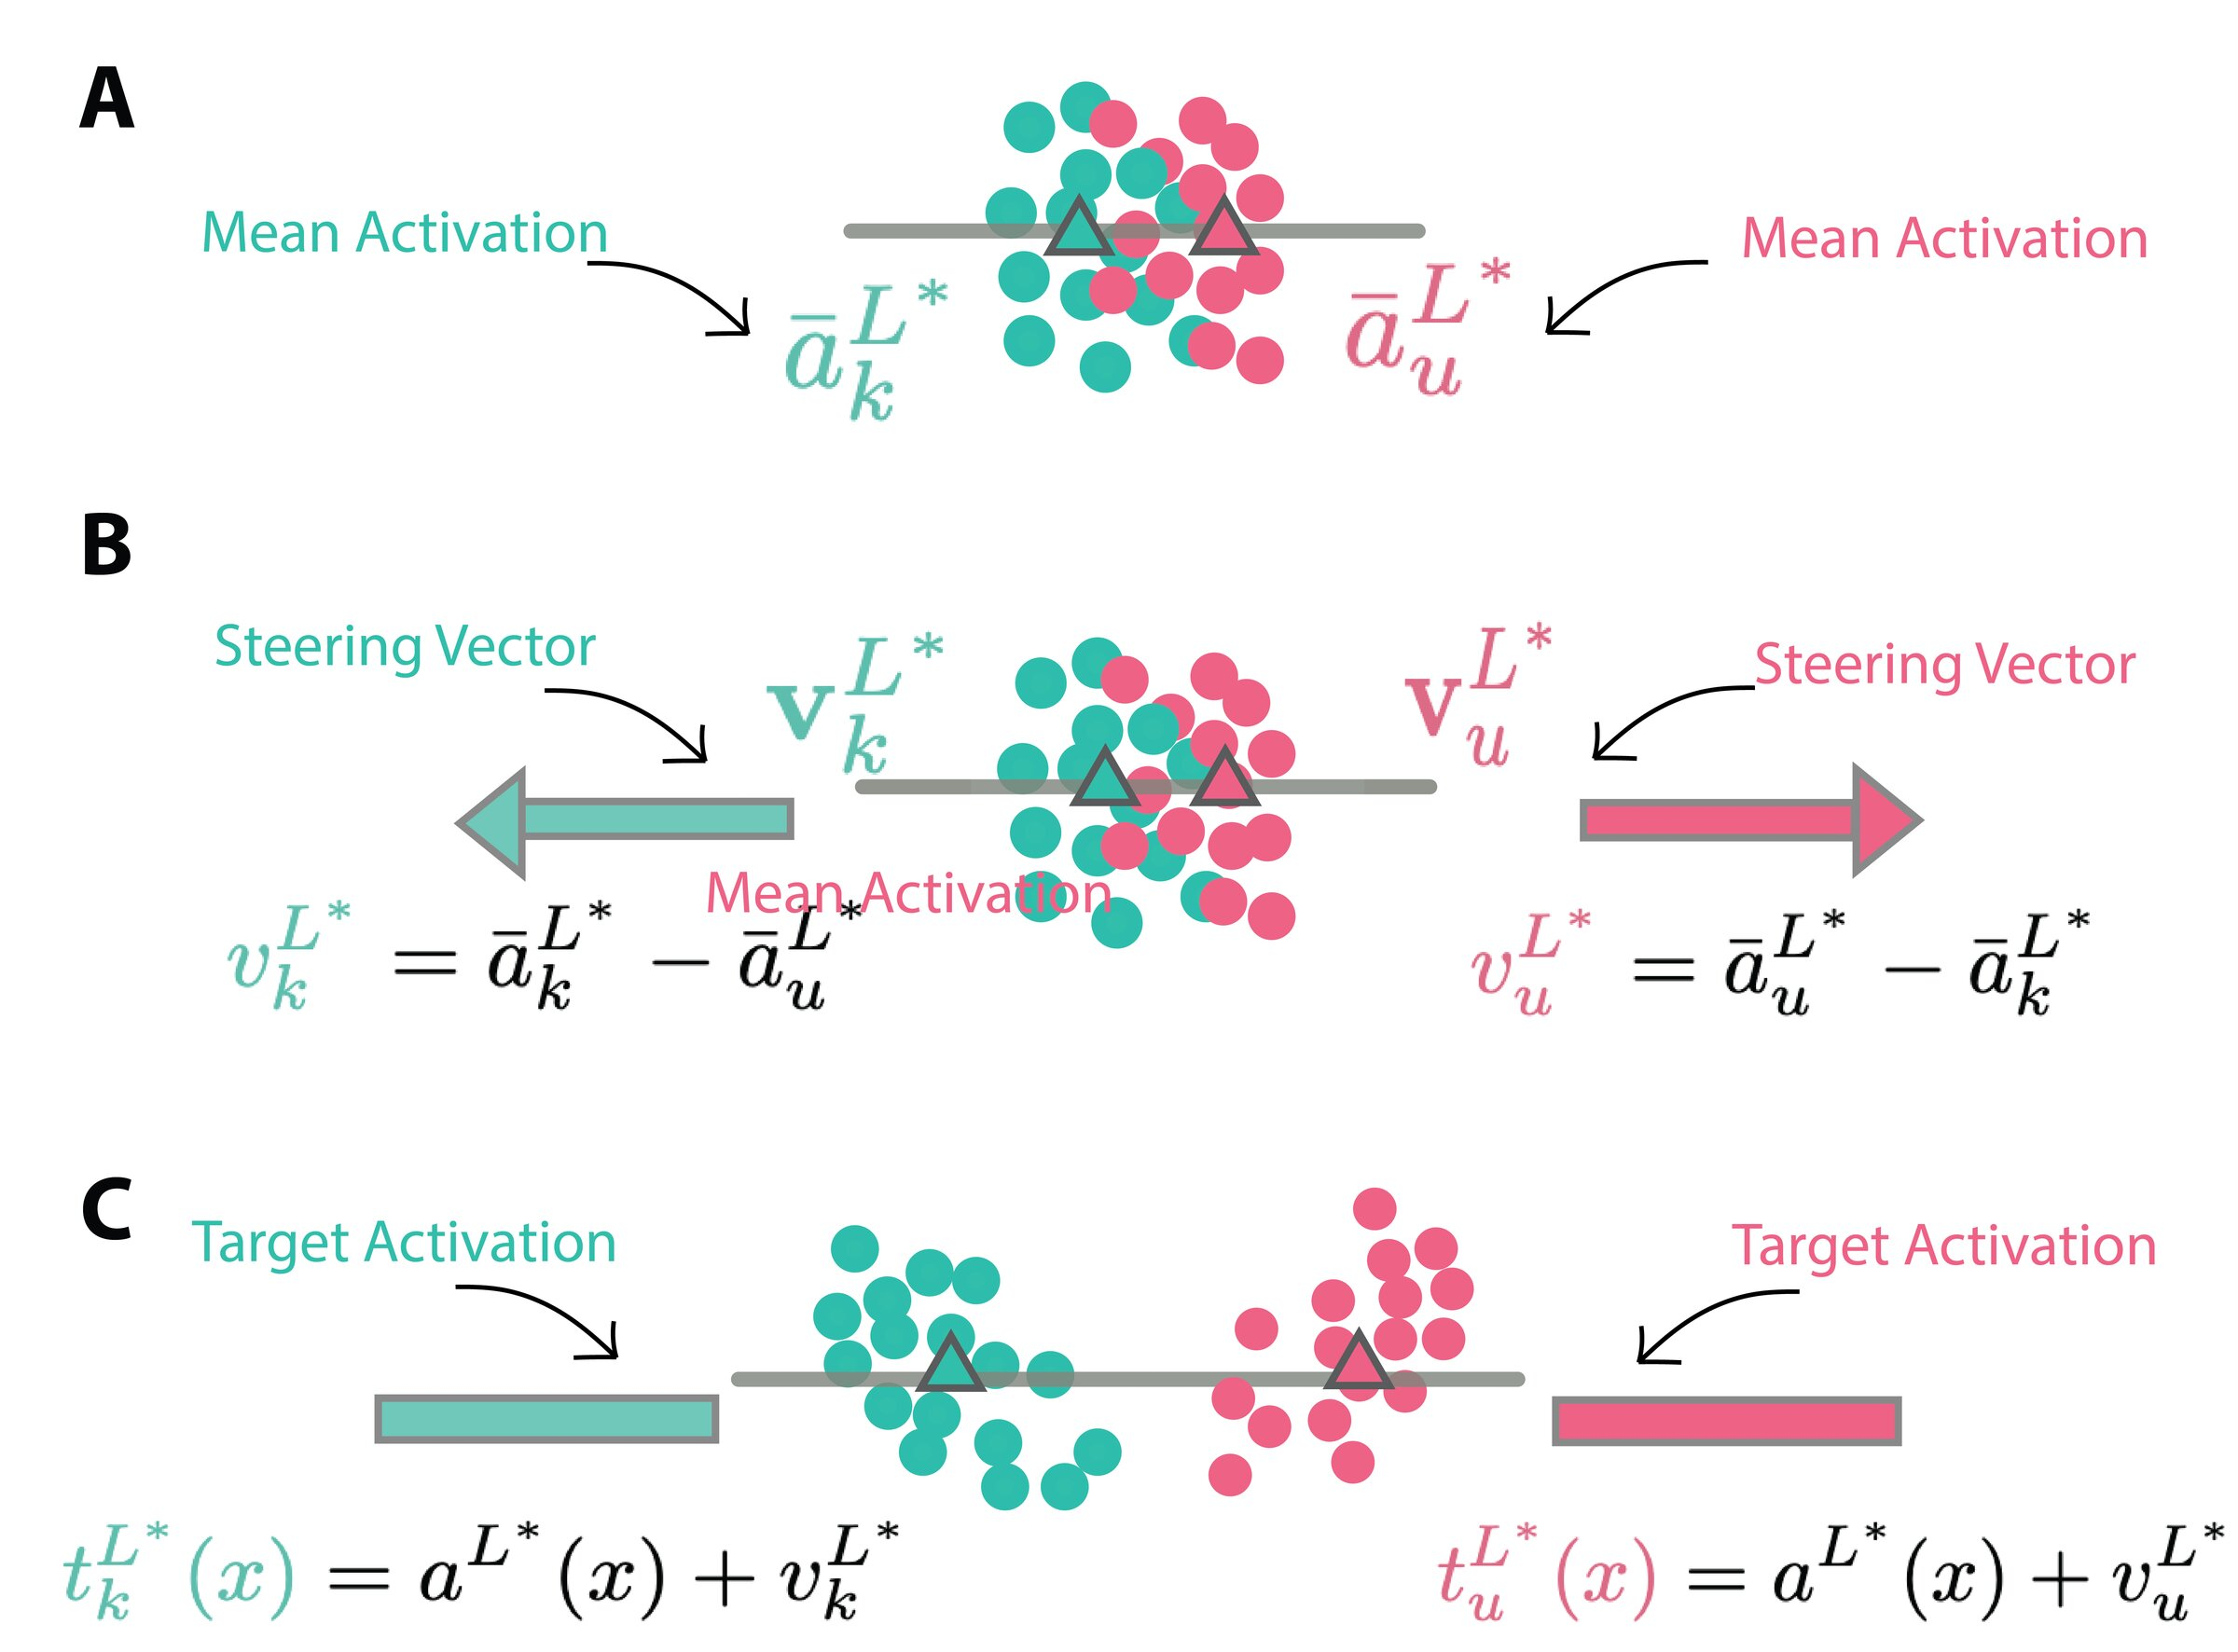
\includegraphics[width=0.75\linewidth]{figures/ch_casal/method_steering.jpg}
    \caption[Steering vector and target activation construction]{%
    \textbf{Illustration of steering vector and target activation construction.}
    (A) Mean activations at target layer $L^*$ are computed for \known{known} and \unknown{unknown} queries.
    (B) Steering vectors are defined by the difference of means, pointing toward the \known{known} or \unknown{unknown} cluster.
    (C) Target activations are generated by shifting raw activations along the corresponding steering vector. These target activations serve as supervision signals during CASAL training.}
    \label{fig:casal_si_steering}
\end{figure}

\paragraph{Layer selection.}
To identify the optimal target layer $L^*$, we apply activation steering at different candidate layers and evaluate resulting generations using two complementary metrics: (1) the hallucination score on \unknown{$\mathcal{D}_u$} (unknown queries), and (2) the accuracy on \known{$\mathcal{D}_k$} (known queries). The optimal $L^*$ is chosen as the layer that simultaneously minimizes hallucination for unknowns while preserving high accuracy for knowns.

% -------------------------
\subsection*{Appendix B: Relationship Between Activation Steering and CASAL Training}
\label{app:casal_training_detail}

\begin{figure}[htbp]
    \centering
    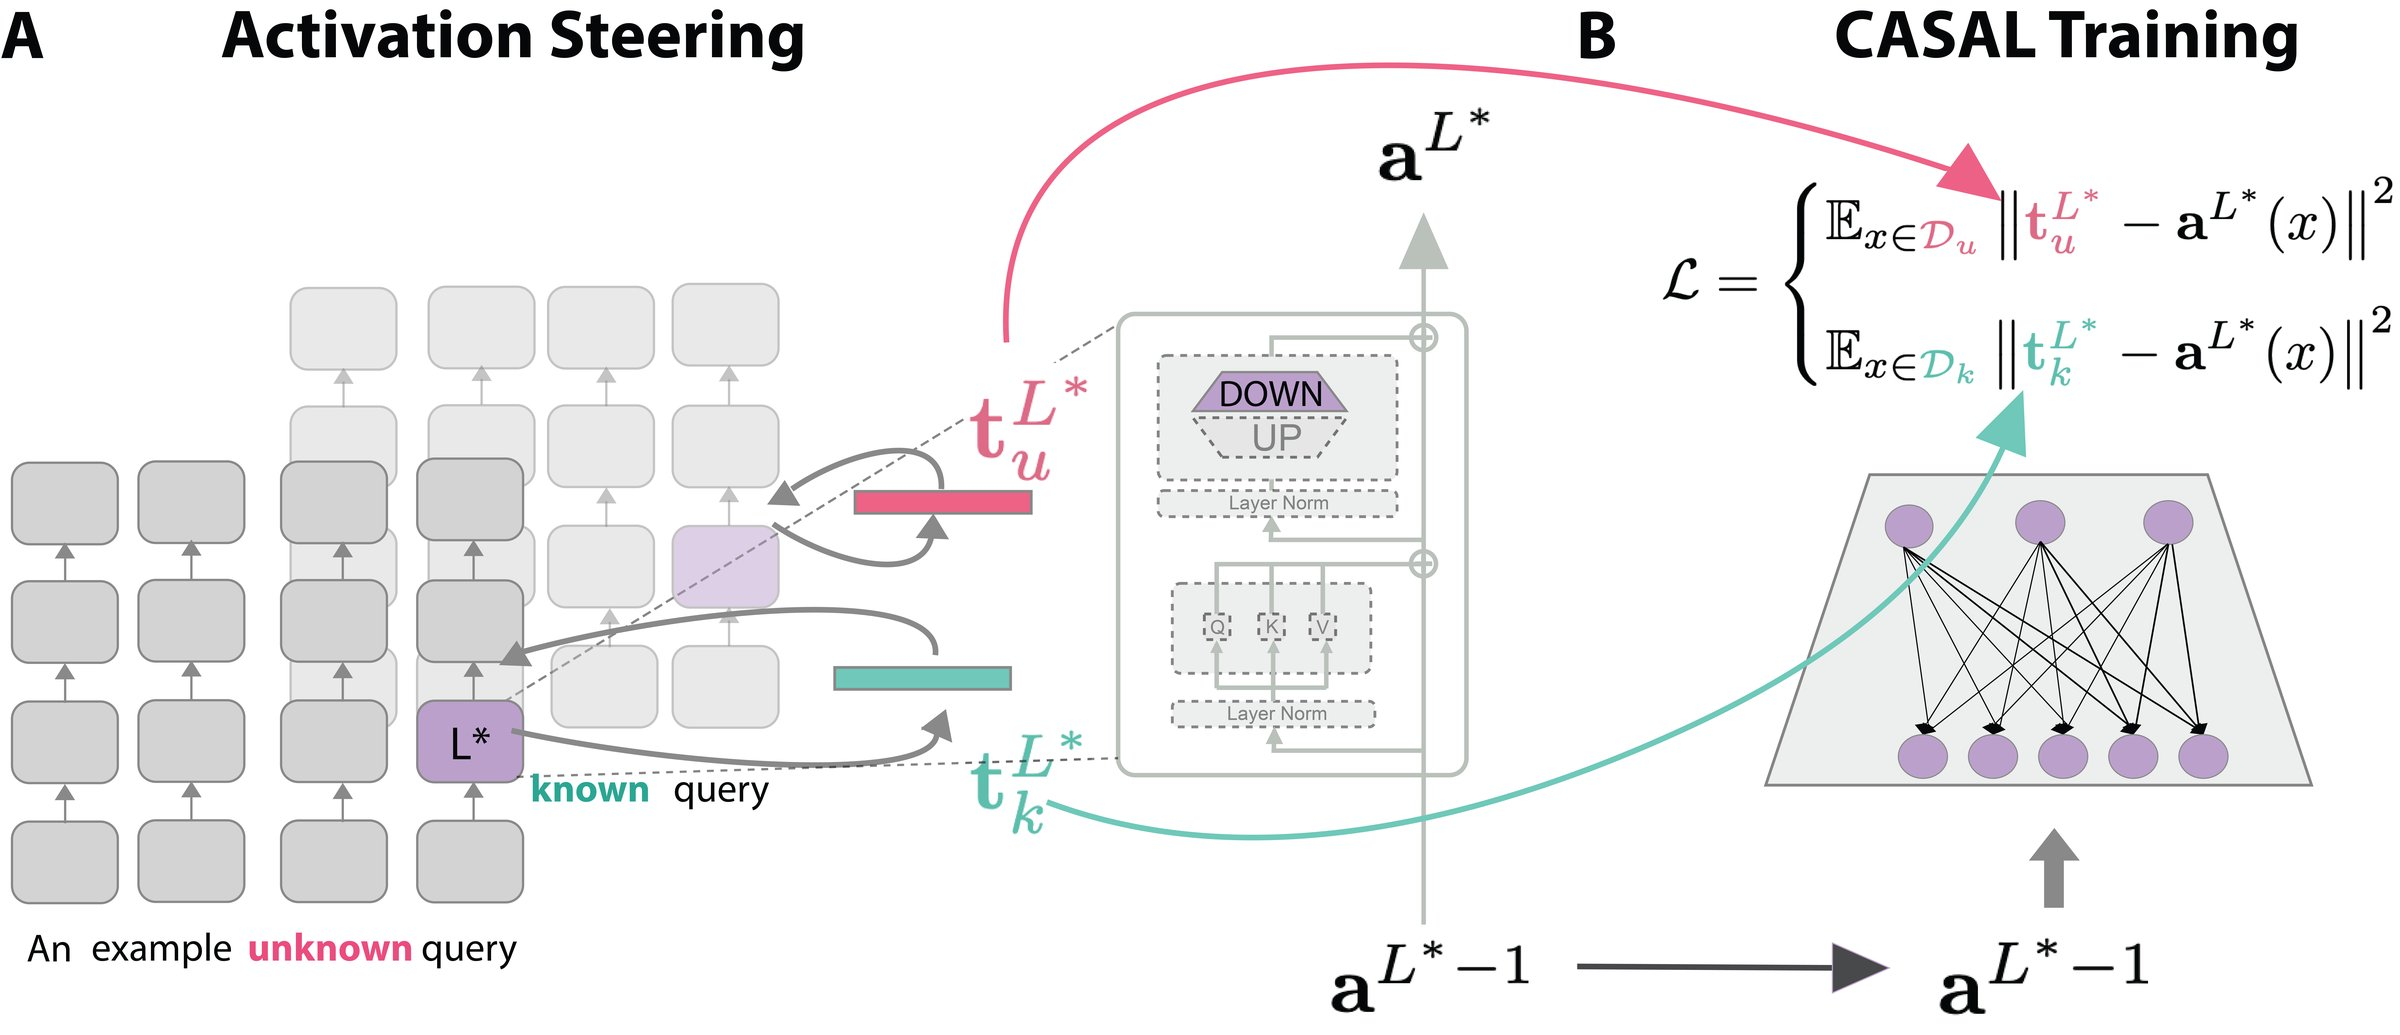
\includegraphics[width=\linewidth]{figures/ch_casal/method_steering_training.jpg}
    \caption[Relationship between activation steering and CASAL training]{%
    \textbf{Relationship between activation steering and CASAL training.}
    (A) \textbf{Activation Steering.} At target layer $L^*$, activations for \known{known} and \unknown{unknown} queries are separated by computing mean representations across each group. Their difference defines steering vectors, applied to produce target activations $\known{t^{L^*}_k(x)}$ and $\unknown{t^{L^*}_u(x)}$.
    (B) \textbf{CASAL Training.} Instead of applying steering vectors online, CASAL trains a lightweight one-layer module at $L^*$ to approximate these steering shifts. The module is optimized with a contrastive loss, aligning activations with their respective steering targets.}
    \label{fig:casal_si_steering_training}
\end{figure}

CASAL can be viewed as an amortized version of activation steering: instead of repeatedly applying steering vectors at inference time, CASAL trains a lightweight module that learns to approximate the steering solution offline and embeds it into the model's weights. The contrastive loss is:
\[
\mathcal{L} =
\mathbb{E}_{x \in \unknown{\mathcal{D}_u}}\|\unknown{t^{L^*}_u(x)} - a^{L^*}(x)\|^2
\;+\;
\mathbb{E}_{x \in \known{\mathcal{D}_k}}\|\known{t^{L^*}_k(x)} - a^{L^*}(x)\|^2 .
\]

% -------------------------
\subsection*{Appendix C: Weight Update Before and After CASAL}
\label{app:casal_before_after}

\begin{figure}[htbp]
    \centering
    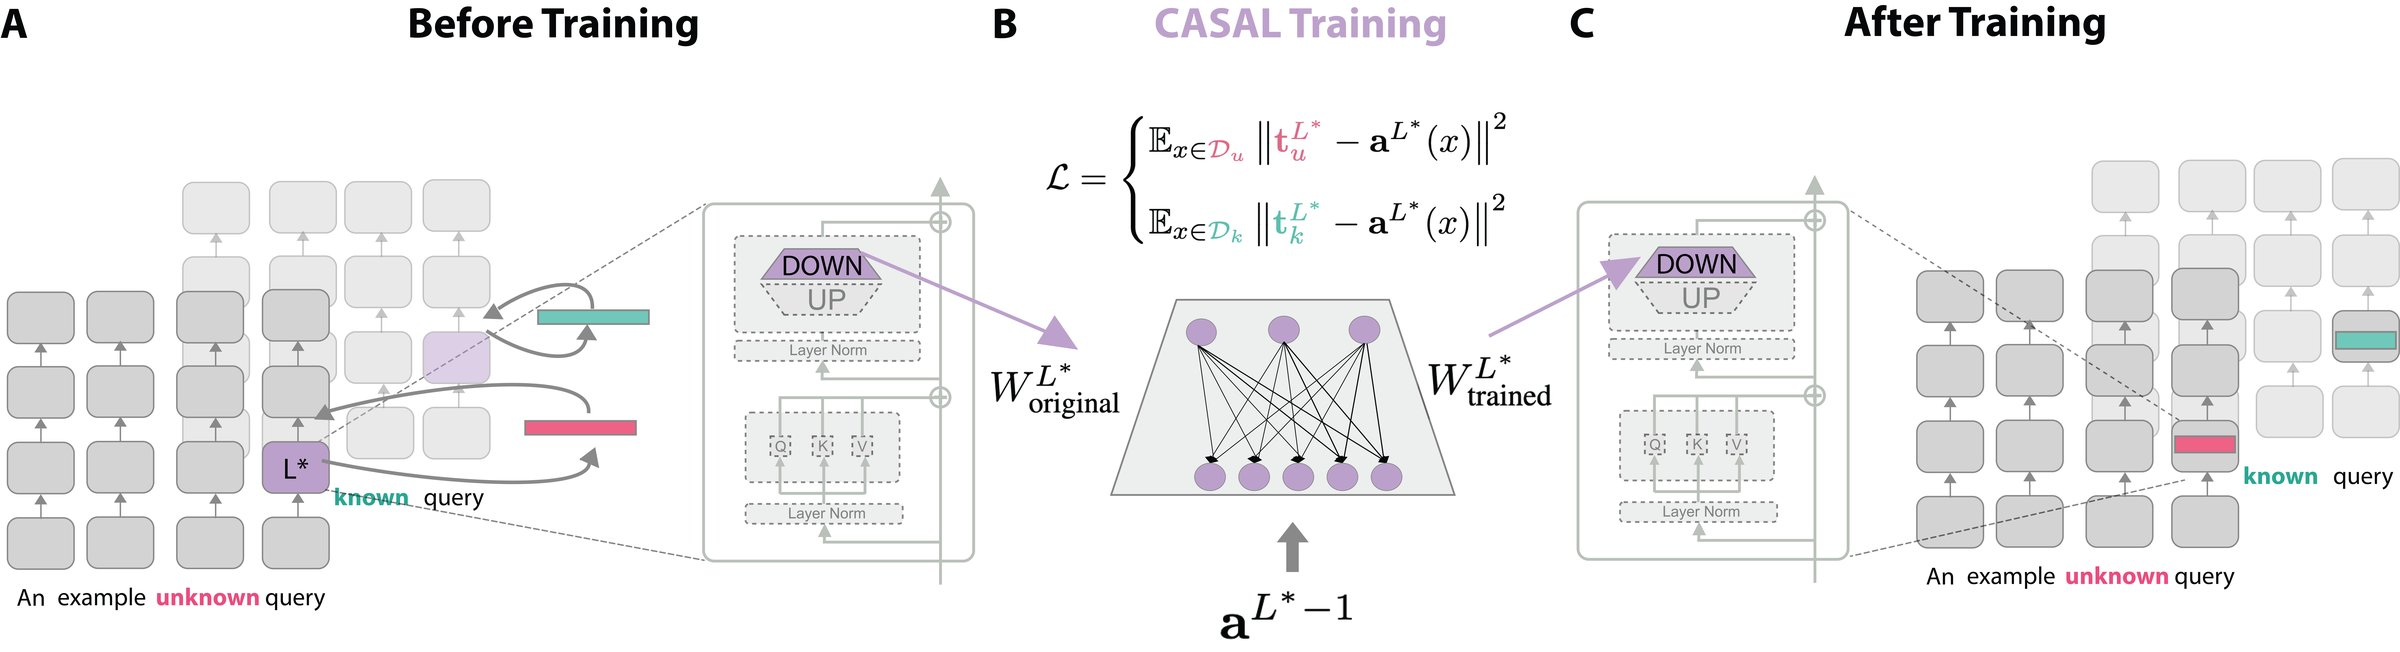
\includegraphics[width=\linewidth]{figures/ch_casal/method_before_after.jpg}
    \caption[Weight update procedure before and after CASAL training]{%
    \textbf{Weight update before and after CASAL training.}
    Before training (Panel A): the frozen pretrained model uses the original weight $W^{L^*}_{\text{original}}$ at the target layer. During CASAL training (Panel B): a lightweight one-layer network initialized from $W^{L^*}_{\text{original}}$ maps pre-activations to updated activations, trained with the contrastive loss to yield trained weights $W^{L^*}_{\text{trained}}$. After training (Panel C): the learned weights replace $W^{L^*}_{\text{original}}$ in the transformer. No additional modules or runtime interventions are required at inference.}
    \label{fig:casal_si_before_after}
\end{figure}

% -------------------------
\subsection*{Appendix D: Contrastive Activation Addition (CAA) vs.\ CASAL}
\label{app:casal_caa}

\begin{figure}[htbp]
    \centering
    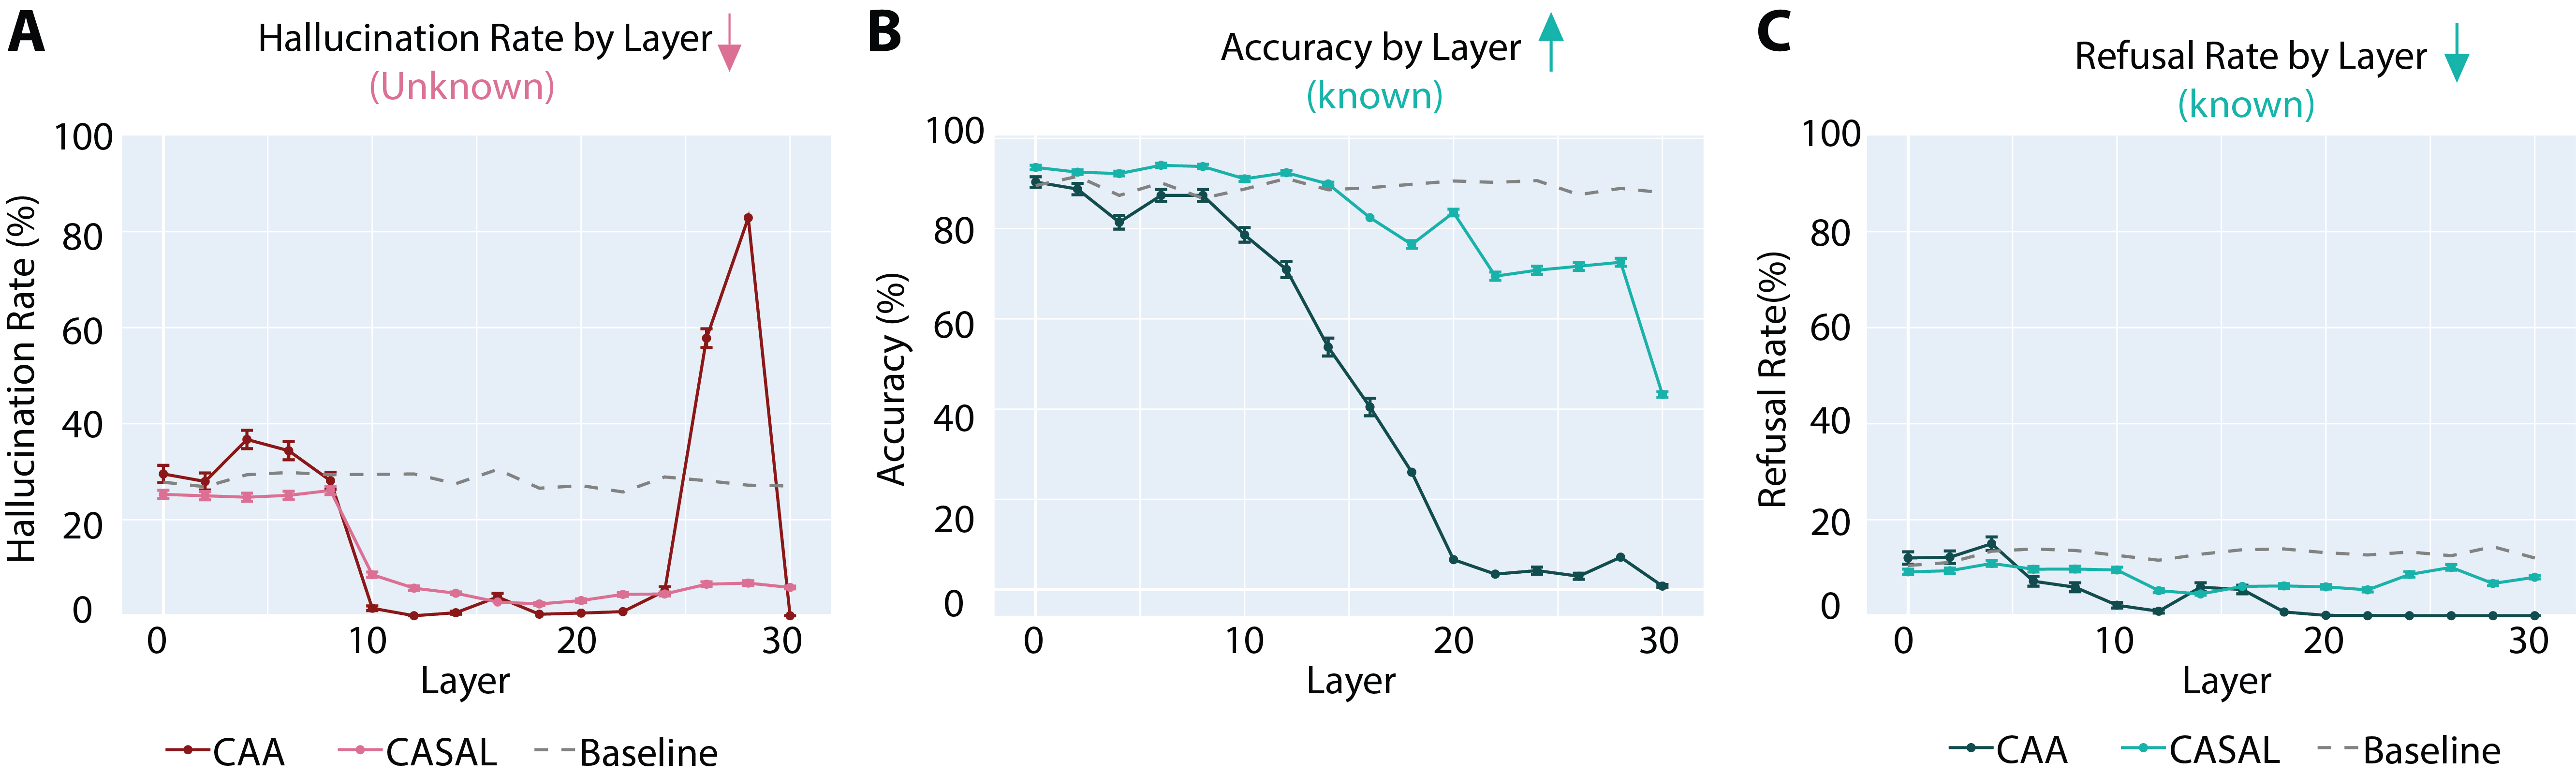
\includegraphics[width=\linewidth]{figures/ch_casal/steering_vs_training/CAA_CASAL_comparison.png}
    \caption[Layer-wise comparison of CASAL and CAA performance]{%
    \textbf{Layer-wise comparison of CASAL and CAA performance.}
    (A) \textbf{Hallucination Rate by Layer (for \unknown{unknown} queries)}: Both CASAL and CAA effectively reduce hallucination rates compared to baseline across most layers.
    (B) \textbf{Accuracy by Layer (for \known{known} queries)}: CAA shows substantial accuracy degradation on known queries at later layers (dropping to $\sim$10\% by layer 30), while CASAL maintains high accuracy ($\sim$70--80\%) across middle layers.
    (C) \textbf{Refusal Rate by Layer (for \known{known} queries)}: Both methods exhibit low refusal rates for known queries across layers. CASAL's superior balance between reducing hallucinations and maintaining performance on known questions makes it significantly more suitable for production deployment.}
    \label{fig:casal_si_caa}
\end{figure}

CAA \citep{contrastive_activation_addition} also adds contrastive directions in activation space to steer model behavior. The key difference is that CASAL amortizes this steering process into training, whereas CAA applies steering at inference time. While both methods effectively reduce hallucination rates on unknown queries, CAA exhibits substantial performance degradation on known queries (accuracy dropping from $\sim$90\% to $\sim$10\% by layer 30), consistent with previous work showing that inference-time steering can introduce undesirable side effects \citep{durmus2024steering, chen2025personavectors}.

% -------------------------
\subsection*{Appendix E: PCA of Activations After Different Training Methods}
\label{app:casal_pca}

\begin{figure}[htbp]
    \centering
    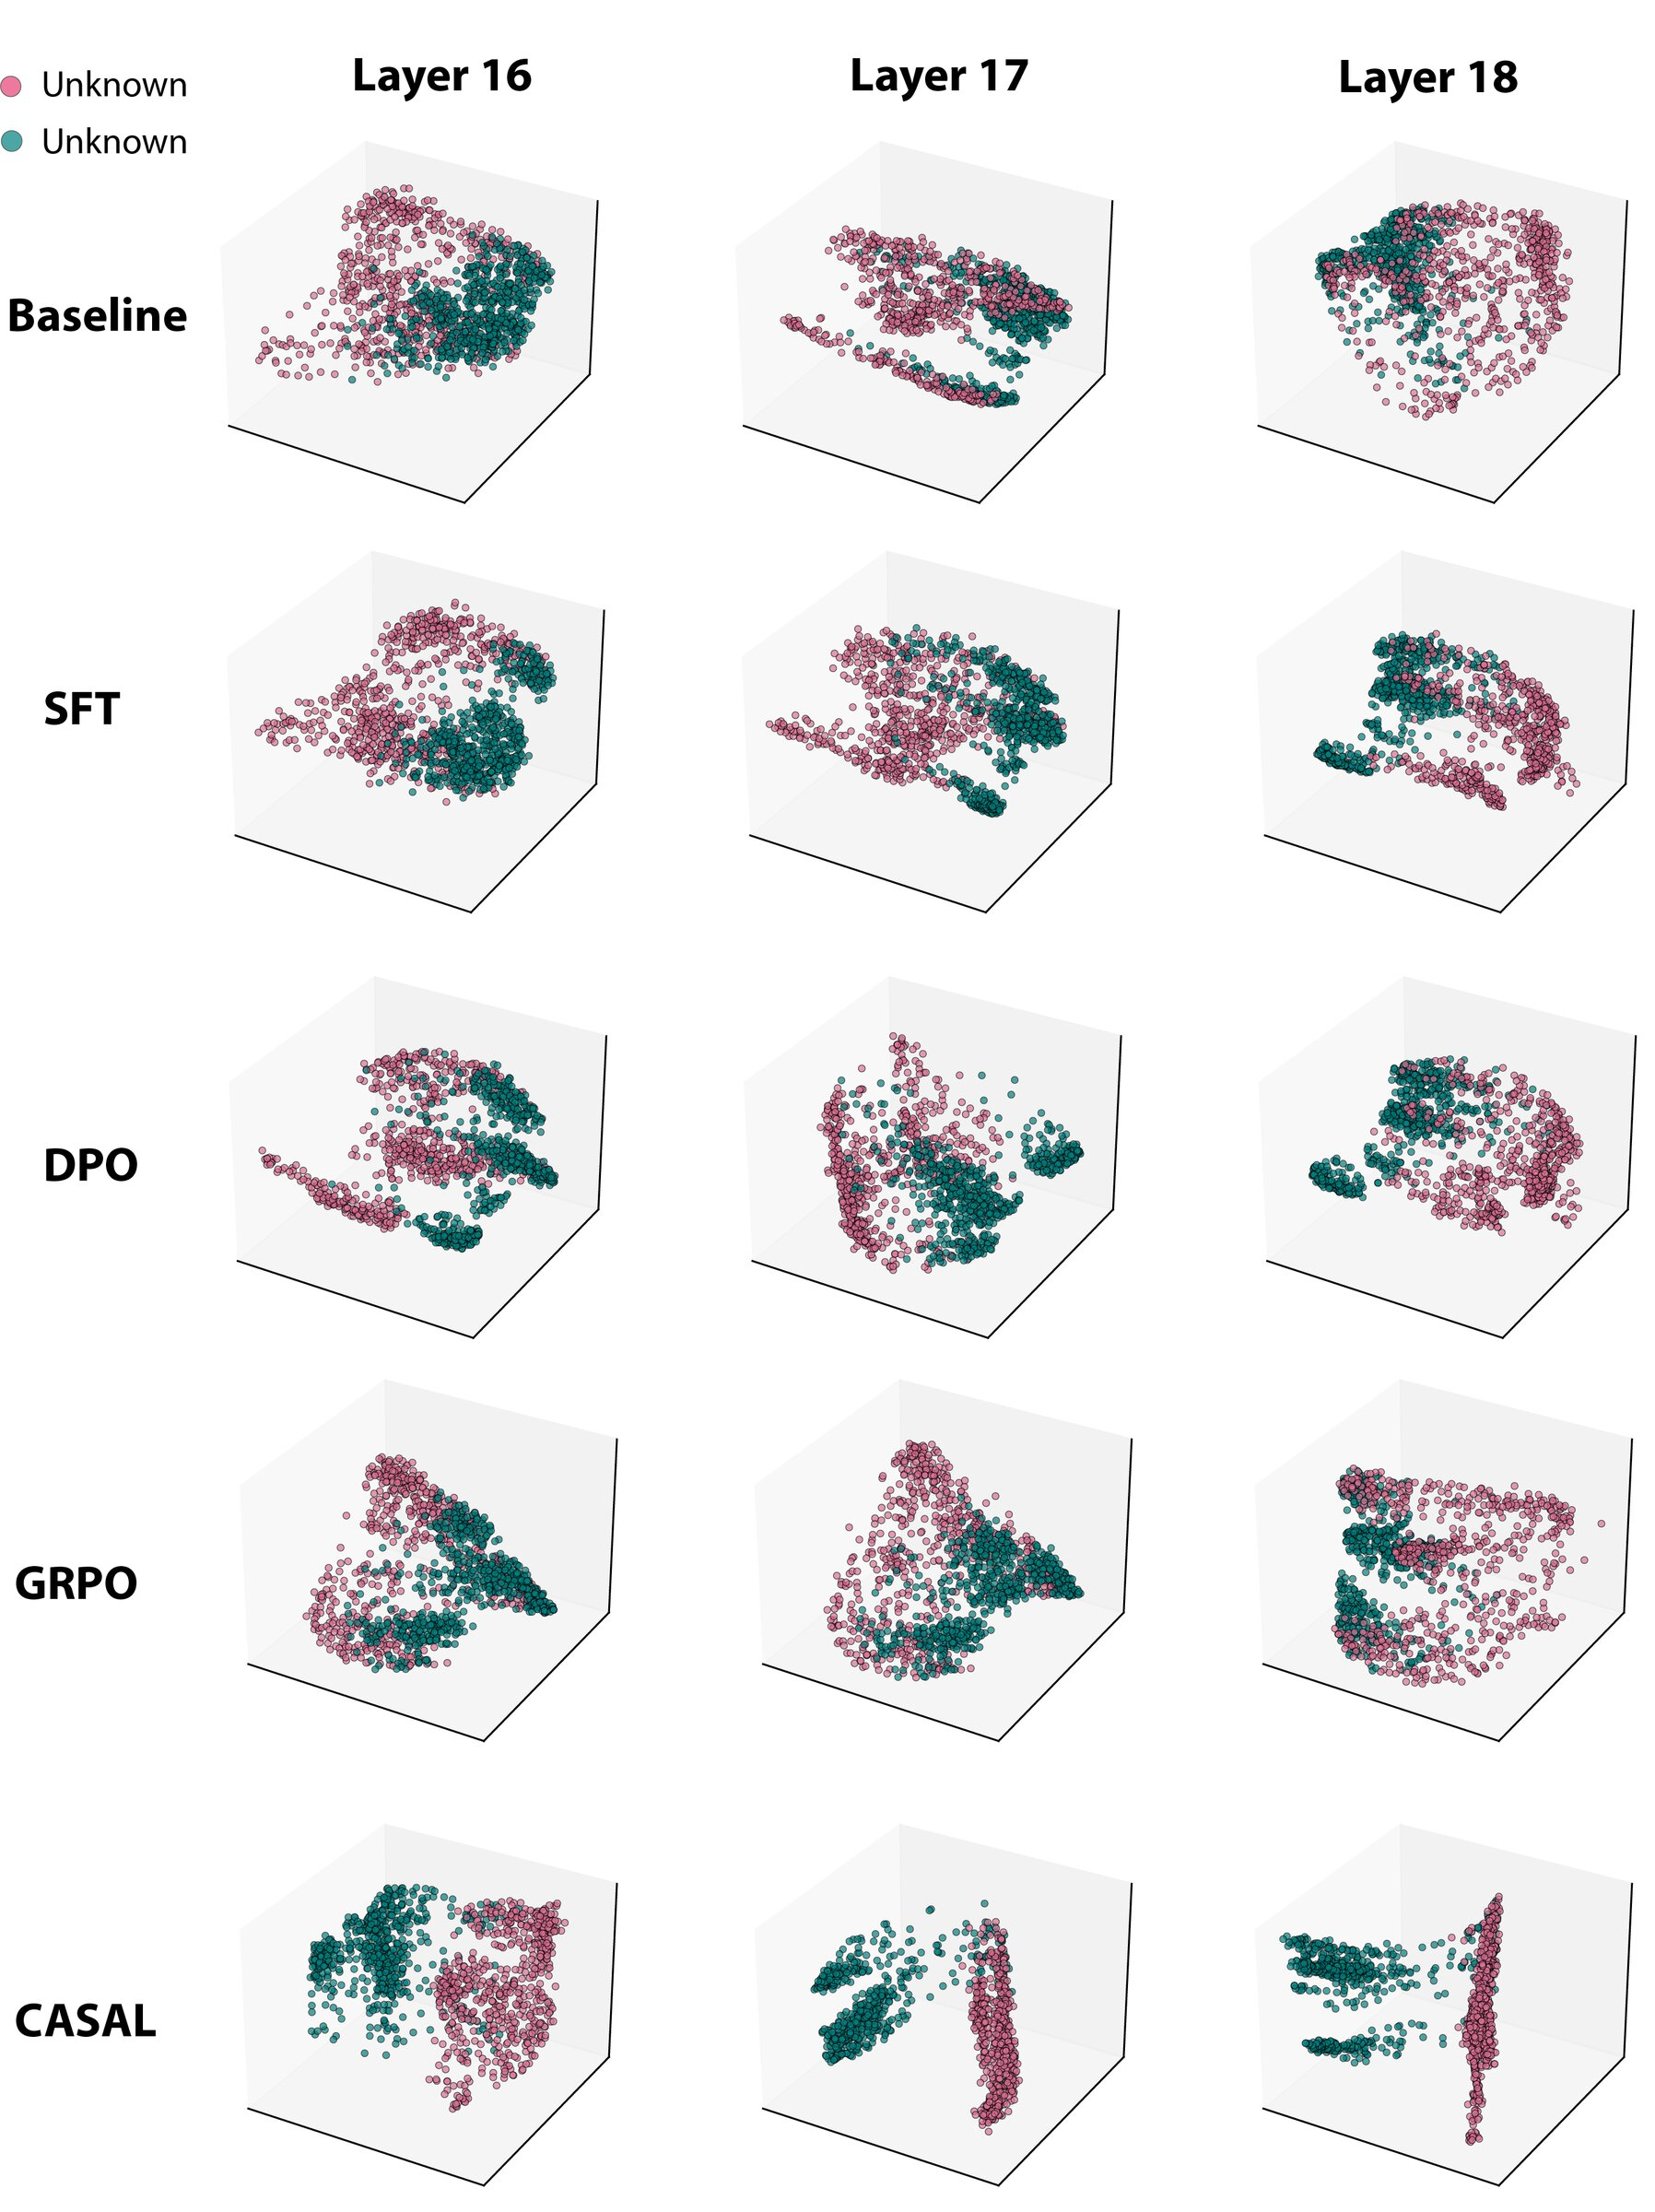
\includegraphics[width=\linewidth]{figures/ch_casal/pca/pca_all.jpg}
    \caption[PCA of residual stream activations after different training methods]{%
    \textbf{PCA of residual stream activations for different training methods.} Each point represents a query, colored by whether the model classifies it as \known{known} (green) or \unknown{unknown} (red). CASAL (rightmost) demonstrates the clearest separation between known and unknown query clusters, validating that the local representation loss directly improves knowledge boundary encoding compared to cross-entropy-based fine-tuning methods.}
    \label{fig:casal_si_pca}
\end{figure}

% -------------------------
\subsection*{Appendix F: Ablation -- Sub-module for Training}
\label{app:casal_ablation}

\begin{figure}[htbp]
    \centering
    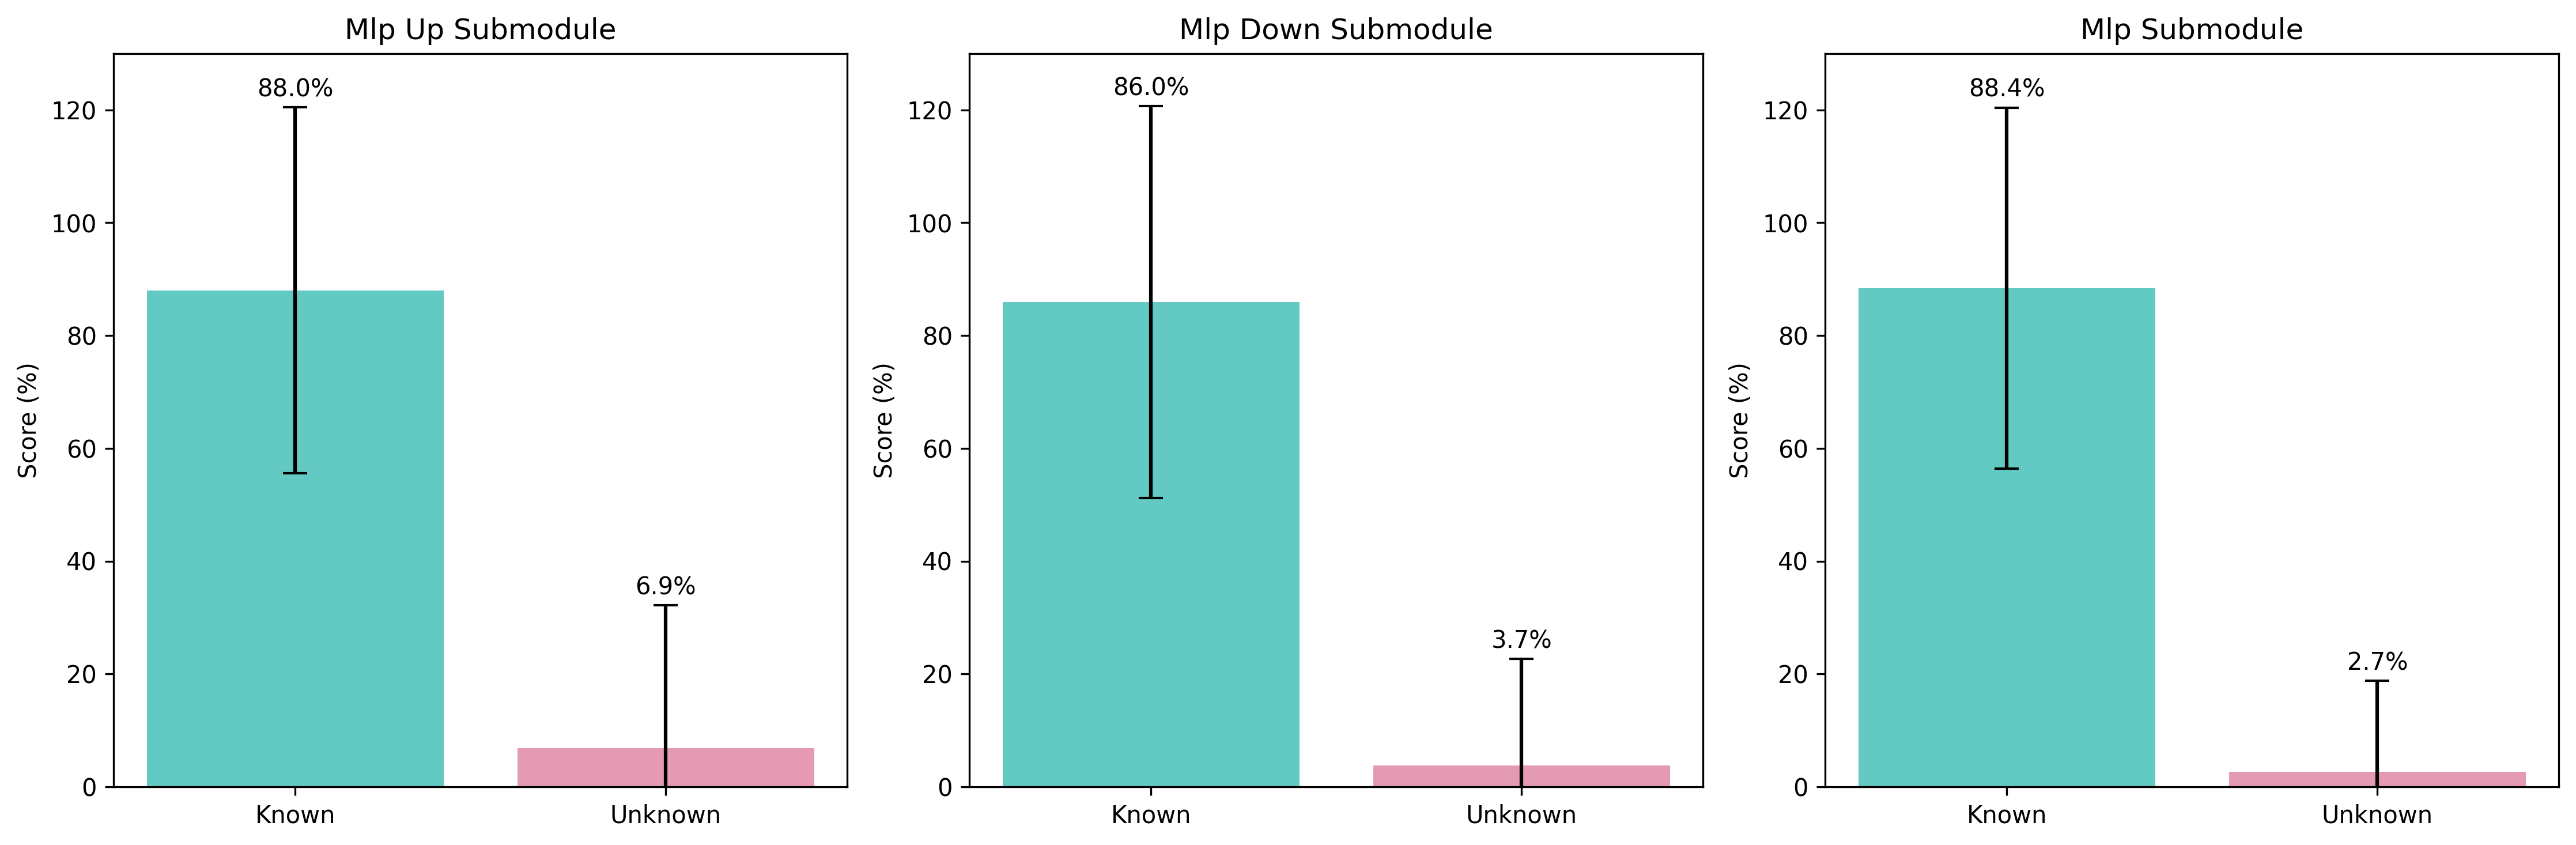
\includegraphics[width=0.75\linewidth]{figures/ch_casal/submodule/submodule_comparison.png}
    \caption[Ablation of MLP submodule selection for CASAL training]{%
    \textbf{Ablation of MLP submodule selection.} Fine-tuning different submodules of the MLP layer (full MLP, up-projection, down-projection) yields no statistically significant performance differences, demonstrating that CASAL's effectiveness is robust to which specific component is updated within the target layer.}
    \label{fig:casal_si_submodule}
\end{figure}

% -------------------------
\subsection*{Appendix G: Hyperparameter Search}
\label{app:casal_hyper}

\paragraph{Learning rate.}
\begin{figure}[htbp]
    \centering
    
\includegraphics[width=0.6\linewidth]{figures/ch_casal/lr/lr.png}
    \caption[Learning rate sensitivity for CASAL training]{%
    \textbf{Learning rate sensitivity.} CASAL hallucination reduction performance across different learning rates. Performance is stable across a broad range, with optimal results at $10^{-4}$--$10^{-3}$.}
    \label{fig:casal_si_lr}
\end{figure}

\paragraph{Steering strength.}
\begin{figure}[htbp]
    \centering
    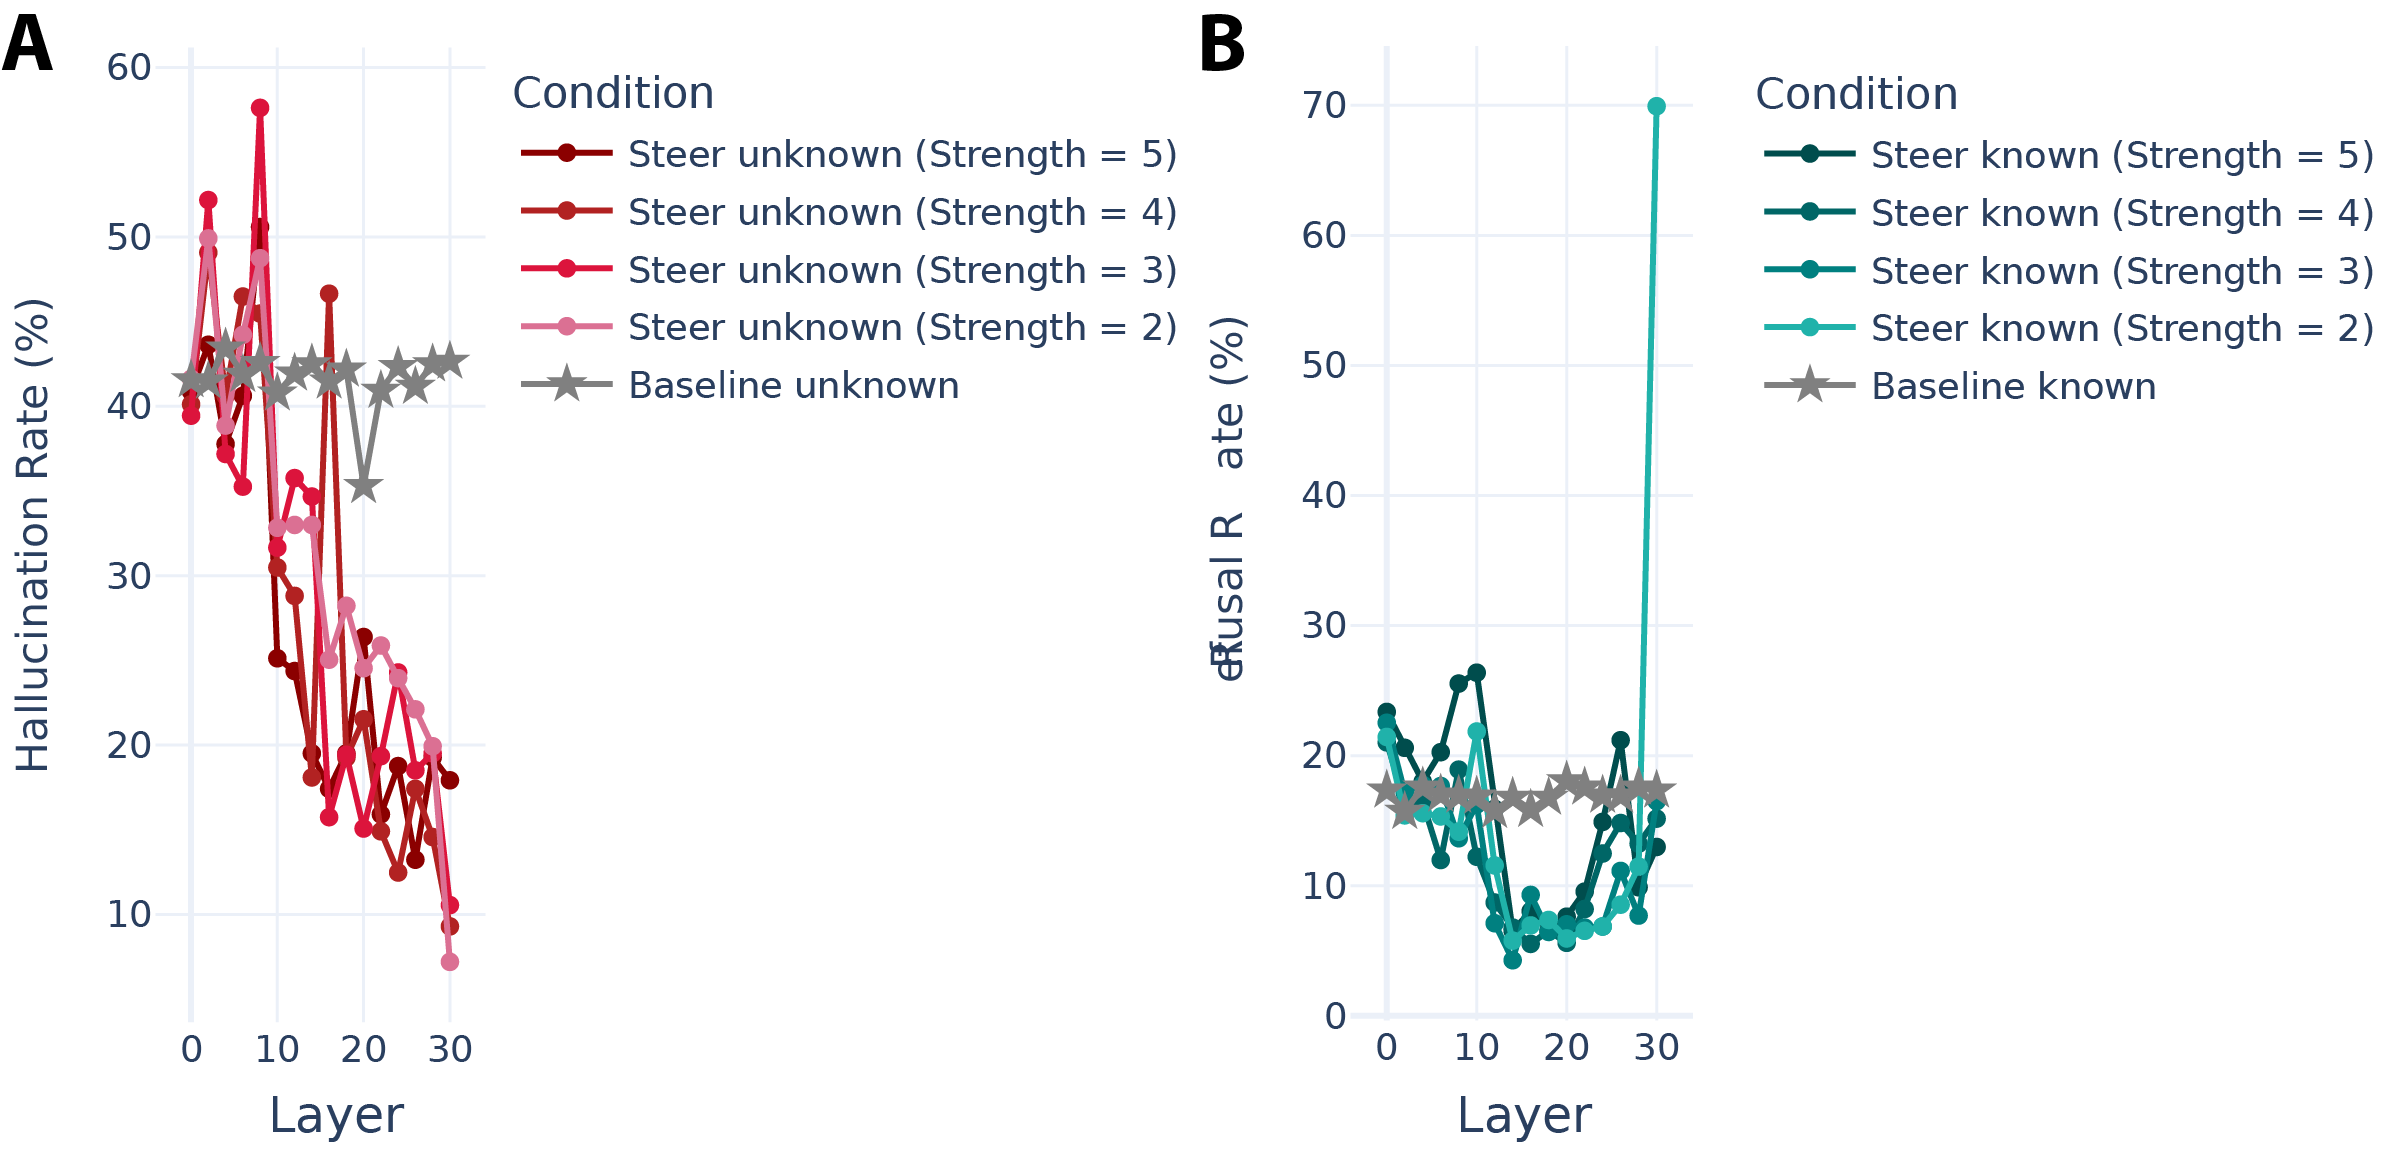
\includegraphics[width=0.6\linewidth]{figures/ch_casal/steering_strength/strength.png}
    \caption[Steering strength sensitivity for CASAL training]{%
    \textbf{Steering strength sensitivity.} Hallucination reduction performance across different values of the steering strength hyperparameter $\alpha$. Performance is robust across a moderate range of steering strengths, with degradation at extremes.}
    \label{fig:casal_si_strength}
\end{figure}

% -------------------------
\subsection*{Appendix H: MoE Training Details -- PCA Activation Across Experts}
\label{app:casal_moe}

\begin{figure}[htbp]
    \centering
    \begin{minipage}[t]{0.32\textwidth}
        \centering
        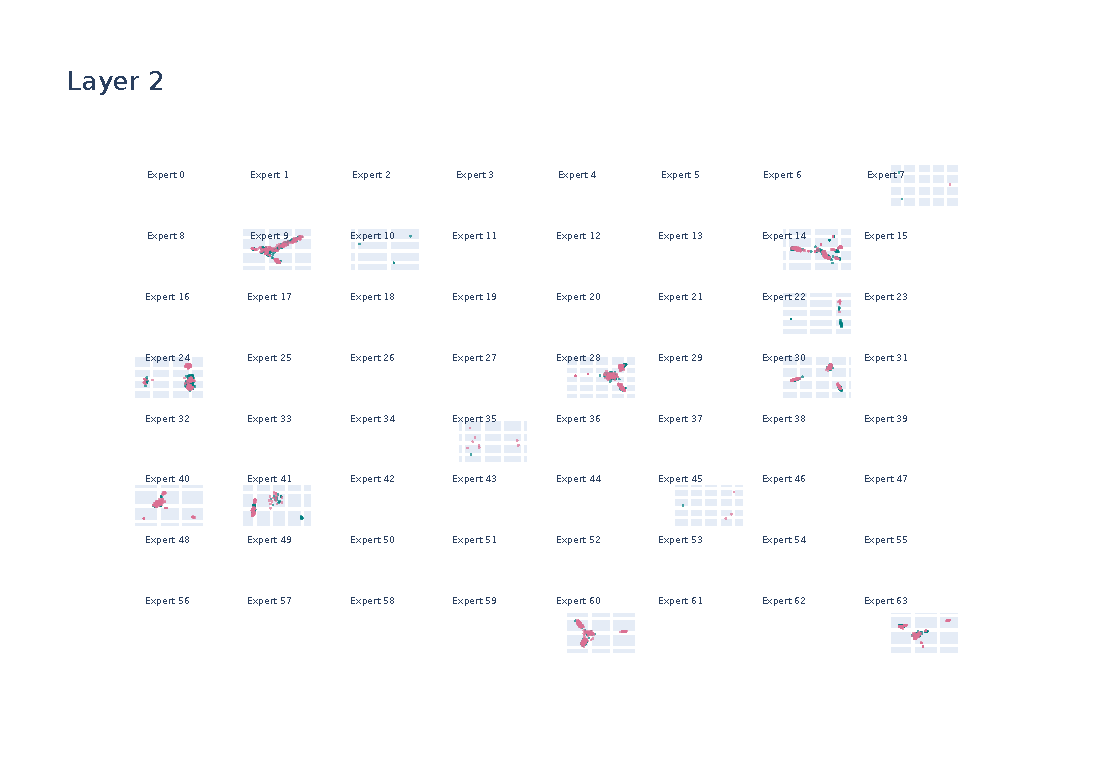
\includegraphics[width=\linewidth]{figures/ch_casal/moe/layer_2_expert_sample_pca_activations_all.pdf}
    \end{minipage}
    \hfill
    \begin{minipage}[t]{0.32\textwidth}
        \centering
        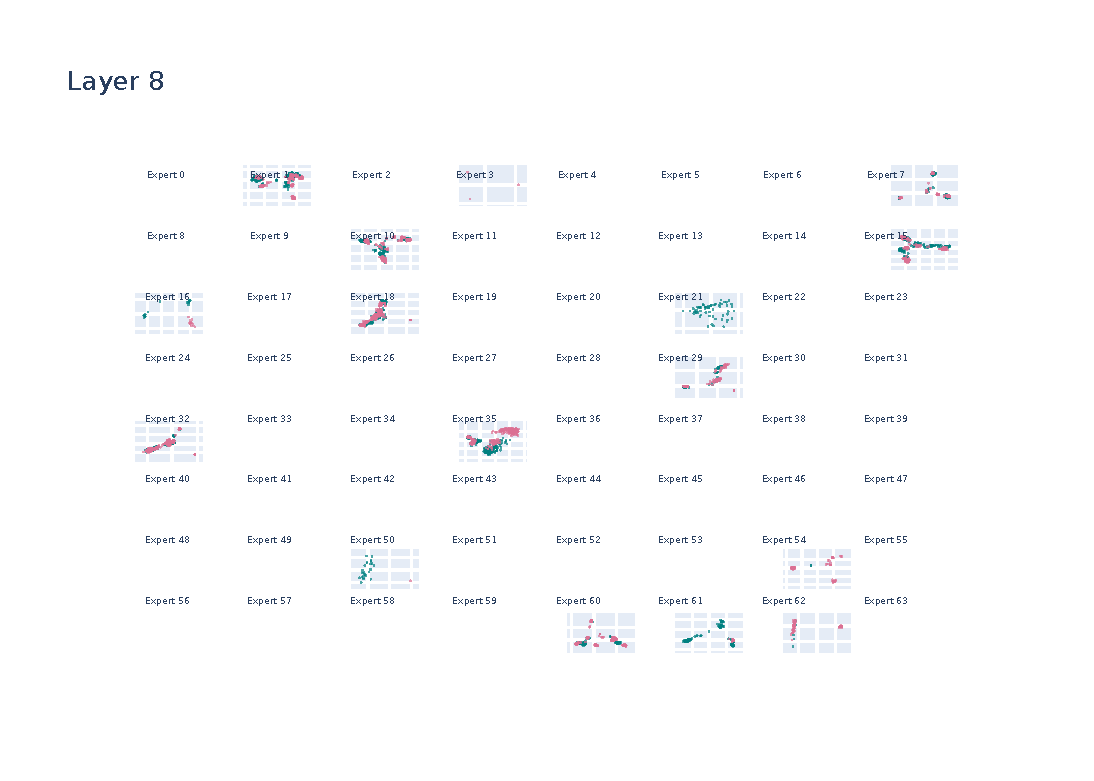
\includegraphics[width=\linewidth]{figures/ch_casal/moe/layer_8_expert_sample_pca_activations_all.pdf}
    \end{minipage}
    \hfill
    \begin{minipage}[t]{0.32\textwidth}
        \centering
        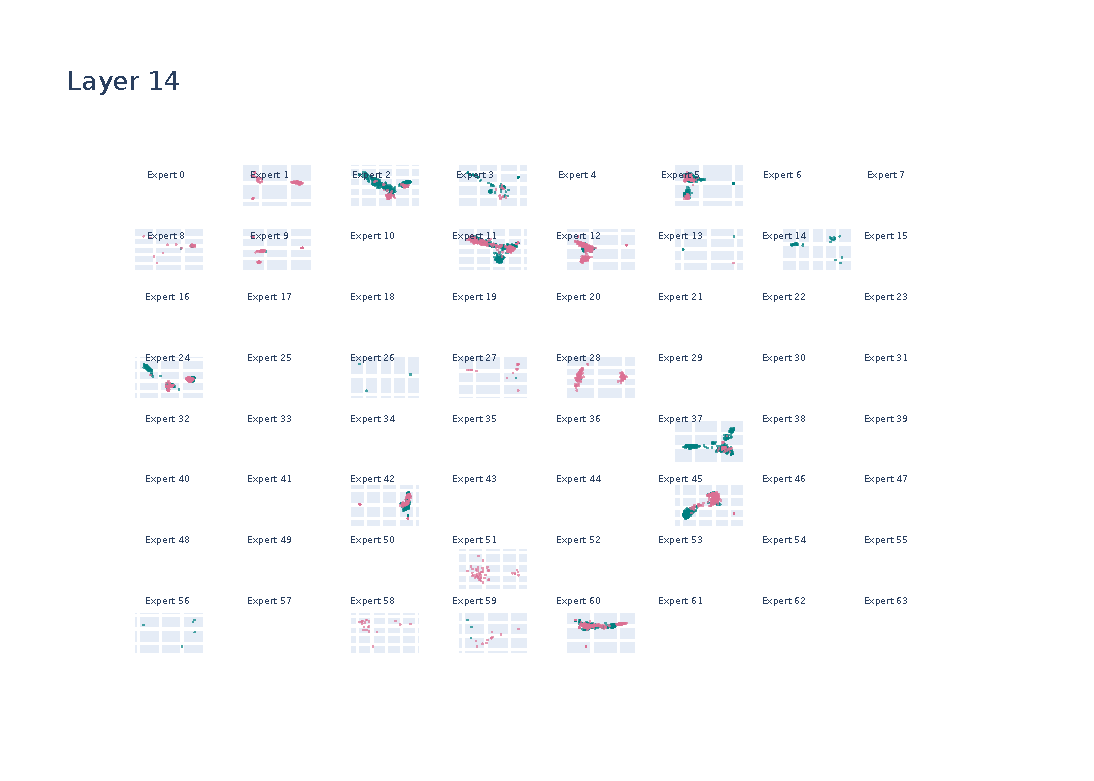
\includegraphics[width=\linewidth]{figures/ch_casal/moe/layer_14_expert_sample_pca_activations_all.pdf}
    \end{minipage}
    \caption[PCA of expert activations in MoE model across layers]{%
    \textbf{PCA of expert activations across layers (2, 8, 14) in the OLMoE model.} \known{Known} (green) and \unknown{unknown} (red) queries are co-represented in the same experts across layers, rather than being routed to specialized experts. This motivates CASAL's approach of applying a global residual stream representation loss rather than expert-specific interventions.}
    \label{fig:casal_si_moe_pca}
\end{figure}

% -------------------------
\subsection*{Appendix I: Knowledge Probing Threshold}
\label{app:casal_probing}

The knowledge probing threshold $\tau$ determines how strictly queries are classified as known vs.\ unknown. We systematically evaluated threshold values in the range $[5, 9]$ (out of $k=10$ samples) and found that hallucination reduction performance remains robust across this range. We adopt $\tau=7$ in all experiments to ensure high-confidence classification: the model abstains only on knowledge it does not possess with high certainty, and responds only when it demonstrates consistent correctness.
